\documentclass[14pt]{report}

\usepackage[english]{babel}

\usepackage{amsmath}
\usepackage{graphicx}

\usepackage[letterpaper,includeheadfoot,margin=2.54cm]{geometry}



\title{Heist}
\author{The Salty Bunch}

%%\titlehead{\centering\includegraphics[width=6cm]{saltybunchlogo}} %%add salty bunch logo

\begin{document}
\maketitle



\tableofcontents


\chapter{Game Overview}

\section{Game Concept}

\begin{itemize}
    \item Play as one of the four thieves attempting a heist on the Cinque National Bank.
    \item Players must infiltrate the bank, which is rigged with traps and hazards to challenge the player.
    \item Security Drones patrol the bank and will engage in combat with players if detected.
    \item Players will be able to use weapons and traps that are available as pickups across the map to engage in combat with other players or the drones.
    \item The main objective of the player is to reach the vault, then collect as much gold as possible from it, and then escape before the lockdown timer reaches zero.
    \item Player that escapes with the most gold possible wins, players who do not manage to escape before lockdown are not awarded points.
\end{itemize}

\section{Setting}

The game is set in the near future at the Cinque National Bank. The CNB is the biggest and most prestigious bank in the world, equipped with high-level defense mechanisms due to its reputation and several failed attempts at a heist. Four of the best thieves in the world are attempting to successfully pull of the biggest heist in history. Unknown to them, they are not alone.

\section{Feature Set}

\begin{itemize}
    \item General Features
    \begin{itemize}
        \item 4 Different Characters
        \item Multiplayer Split-Screen Game
        \item Pixelated Voxel-Style Art
        \item 3D Isometric
    \end{itemize}
    \item Gameplay
    \begin{itemize}
        \item Combat
        \item Hazards and Traps
        \item Stealth
        \item Enemy Drones
        \item Quick-time Events
        \item Scoring System
    \end{itemize}
\end{itemize}

\section{Genre \& Target Audience}
Heist is a multiplayer action party game, targeted at players ages 13 and above.

\section{Game Flow Summary}

\begin{figure}
	\includegraphics[width=\linewidth]{images\\gameflowsummary.jpg}
	\caption{Game Flow Summary}
	\label{fig:gameflowsummary}
\end{figure}

Figure \ref{fig:gameflowsummary} Shows Game Flow Summary

\section{Look and Feel}

Heist will have a fun, arcadey, but still have a competitive side to it. It will be easy to pickup, with not much complexity to it, and a lot of intuitive mechanics. We will use a pixel low poly art style to represent the environment and the characters in the game.

\begin{figure}
	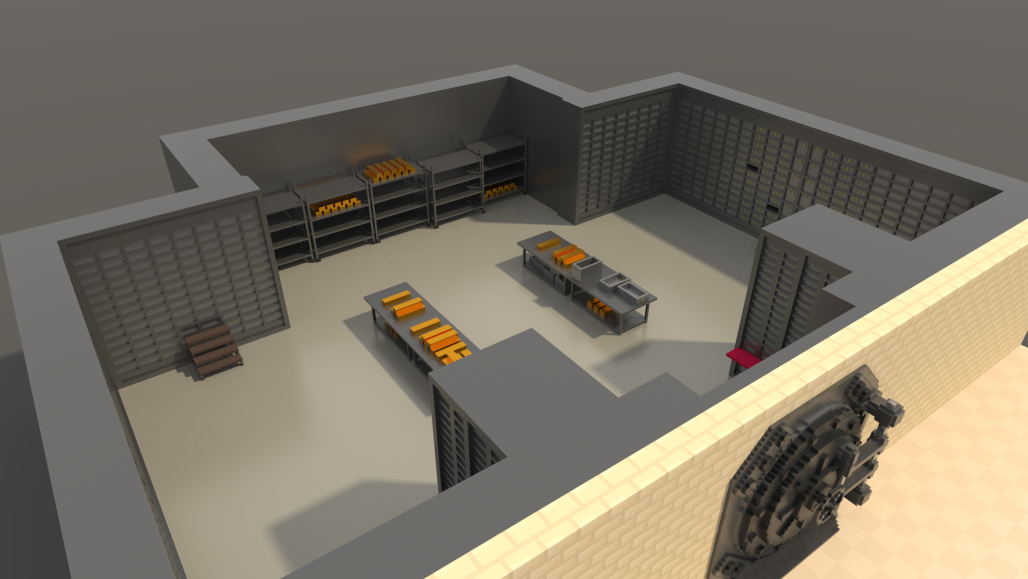
\includegraphics[width=\linewidth]{images\\lookandfeel.png}
	\caption{Look and Feel}
	\label{fig:lookandfeel}
\end{figure}

Figure \ref{fig:lookandfeel} Concept Render Within Vault

\chapter{Story and Setting}

\section{Story and Narrative}

Our setting is the Cinque National Bank (CNB), it is a prestigious and sophisticated bank frequented by the rich and known by thieves as a goldmine. Set in the near future, Cinque National Bank is notorious for their top of the line security and surveillance measures in addition to being loaded.  The bank is a complex building with a lot of hallways, rooms, and sections with state of the art defense and security mechanisms along with professional security drones. Although many thieves from all around the world have attempted to pull off heists, no one has been successful, so far. This time, however, four thieves plan to perform the biggest heist in history at Cinque National Bank, but little do they know, they are all there on the same night.

\subsection{Game Progression Summary}

Four thieves spawn at random at one of the four points of entry. In the first stage, their objective is to infiltrate the bank by getting past quicktime events to bypass traps and hazards. Secondly, they must now move through the bank to not get spotted by other players or security drones. 
Their next objective is to get to the vault and obtain as much gold as possible and more then the next player to win. After they need to obtain as much gold as possible from the bank, they have to escape through the bank from a randomly chosen escape point in the bank before the lockdown timer expires and they get stuck in the bank.

\section{Cut Scenes}
\subsection{(Introduction)}

All four characters are introduced to the player through a slanted comic book style to demonstrate to the player exposition of how the four thieves got to the bank (See concept below). This cutscene is triggered after the players have all selected their characters and enter the game.

\subsubsection{Description}

EXT. Outside of Bank - NIGHT

Four characters are seen on the left side of the screen on one of the slanted comic book-like panels. 
First panel is of the one of the four characters running/sneaking to the bank.
Second panel is one of the four characters staring up at the bank in awe.
	
INT. Inside of Bank - NIGHT

Third panel is one of the four characters breaking/sneaking into the bank.
Last panel is one of the four character gesturing that they are ready to rob the bank.

\subsubsection{Storyboard}
%%TODO (Insert Later)

\subsection{Victory Screen}
%%TODO (Insert Later)

\section{Game World}

\subsection{General Look and Feel of the World}

\subsubsection{Ground Floor}

The ground floor will contain, office spaces, board/conference rooms, teller stations, restrooms, information booths used by the employees of the CNB.

The environment will remain clean and modern with simple geometric shapes i.e. chairs, tables, ATM’s and etc that are found throughout the bank.

\subsubsection{Basement}
%%TODO (TBC)
The basement contains the vault.

\chapter{Characters}
%%HERE I AM

\chapter{Gameplay and Mechanics}

\section{Game Progression}
Game Progression split into 3 parts

\subsection{Infiltration}
\begin{itemize}
    \item Infiltration stage implies that the players must sneak in to the bank and make their way towards the basement.
    \item Infiltration stage will require players to be more stealthy
    \item Players can engage in combat
    \item Players will familiarize themselves with the environment and its challenges in this stage
\end{itemize}
\subsection{Scavenging}
\begin{itemize}
    \item This stage of the game blends between the other two stages
    \item Players will collect weapons and traps
    \item Players will set traps across the map for other players
    \item They will explore rooms and hallways for loot 
\end{itemize}
\subsection{Lockdown}
\begin{itemize}
    \item This stage will be the most chaotic stage of the game
    \item As soon as a player accesses the vault, a lockdown timer initiates
    \item In this stage, players will be rushing and battling to gather as much gold as possible and try to escape the bank before lockdown.
    \item Only one exit will be available
    \item More traps and hazards will spawn
    \item Drones will be more aggressive
\end{itemize}

\section{Objectives}
\subsection{Main Objectives}
\begin{itemize}
    \item Achieve the highest score possible by collecting gold from the vault
    \item Escape before lockdown
\end{itemize}
\subsection{Secondary Objectives}
\begin{itemize}
    \item Dodge and disable traps and hazards
    \item Collect weapons and traps
    \item Use weapons to engage in combat with players and/or drones
    \item Set pick-up-able traps
\end{itemize}

\section{Challenges}
There are multiple challenges for the player
\subsection{Level Layout}
\begin{itemize}
    \item Levels are not going to be straightforward paths towards the vault
    \item Levels will contain multiple paths, each with their own pros and cons
    \item Level of difficulty and frequency of pickups will vary area to area
    \item Hazards will already be set in the map at the beginning of the game
    \begin{itemize}
        \item Laser Tripwire: will inform enemy drones to the players position and send them to the player's area
        \item Electric Field: 
        \item Lethal Lasers: 
    \end{itemize}
    \item Hazards will be strategically set at areas of importance
    \item Some hazards can be disabled temporarily through a quick-time event
    \begin{itemize}
        \item If quick-time event is successful, trap is disabled for a short amount of time
        \item If quick-time event is failed, trap is triggered
    \end{itemize}
\end{itemize}

\subsection{Security Drones}
\begin{itemize}
    \item Drones are the primary enemy for the players
    \item They patrol the bank, and will detect players in their vision radius
    \item Drones will attack the player if a player is detected
    \item Drones will be equipped with either of the following weapons
    \begin{itemize}
        \item Stun Gun: ranged weapon that charges up before firing (dodgeable)
        \item Electric Field: AoE weapon that drones can deploy for short bursts, it deploys an electric field under them that will damage players that step in it. Drones will be faster and chase players around
    \end{itemize}
\end{itemize}

\subsection{Combat}


\section{Play Flow}

\section{Mechanics}
\subsection{Physics}
\subsection{Movement}
\subsection{Score}
\begin{itemize}
    \item Score is calculated post game based on several factors. Either positively or negatively
    \begin{itemize}
        \item Positively
        \begin{itemize}
            \item The amount of gold removed from the bank
            \item Escaping from the bank before lockdown
        \end{itemize}
        \item Negatively
        \begin{itemize}
            \item The number of times the player has been stunned
            \item The amount of time taken to get in and out of the vault
        \end{itemize}
    \end{itemize}
\end{itemize}
\subsection{Objects}
\subsubsection{Traps}
\begin{itemize}
    \item Traps can be found as pickups throughout the level based on a random spawning System
    \begin{itemize}
        \item Found scattered throughout the level, predominately found on the vault floor, but also on the ground floor
    \end{itemize}
\end{itemize}
\subsubsection{Items}
\begin{itemize}
    \item Weapons are found throughout the level, where worse weapons are found on the ground floor and better weapons are found on the vault floor
\end{itemize}
\subsubsection{Gold}
\begin{itemize}
    \item Gold can be found in several places throughout the level
    \item At the beginning all gold will be in piles within the vault
    \item Gold within the vault can be picked up through an interaction that initiates a transfer between the gold pile and the player
    \begin{itemize}
        \item Gold gets transferred at a fixed rate until the pile is empty or the player cancels
        \item Successfully completing quick-time events during the transfer increases the current rate of gold transfer
    \end{itemize}
    \item As players that have gold get damaged by players, drones and traps, their gold gets dropped on the ground
    \begin{itemize}
        \item These small piles of gold can be picked up simply by walking over them.
    \end{itemize}
\end{itemize}
\subsection{Actions}

\section{Combat}

\begin{itemize}
    \item Players will be able to engage in combat with:
    \begin{itemize}
        \item Other player characters
        \item Drones
    \end{itemize}
    \item Players will start with a default melee weapon for each character
    \begin{itemize}
        \item King:
        \item Shadow:
        \item Racoon:
        \item Jailbird:
    \end{itemize}
    \item Player \emph{Weapons} that will be available as pickups across the map:
    \begin{itemize}
        \item \emph{Stun Gun}:
        \begin{itemize}
            \item Shoots a projectile that moves X units in a certain direction
            \item Fire rate at 1 shot/2 seconds
            \item Projectile can be dodged by players or drones
            \item Projectile will do 1 DMG when enemy is highest
            \item Projectile will disappear upon impact
            \item Player gets 6 shots per Stun Gun pickup
            \item After 6 shots, Stun Gun will disappear from inventory
        \end{itemize}
        \item \emph{Electric Baton}
        \begin{itemize}
            \item Melee weapon that increases player movement speed and melee attack range (charge)
            \item Lasts for 20 seconds
            \item Cannot pickup other weapons during Baton `charge'
        \end{itemize}
    \end{itemize}
    \item Player \emph{Traps} that will be available as pickups across the map:
    \begin{itemize}
        \item \emph{Electric Field}:
        \begin{itemize}
            \item Pick up
            \item Can be deployed on any tile (if the tile has no traps already)
            \item AoE damage field
            \begin{itemize}
                \item Does 1 DMG/2 seconds
                \item Slows player movement speed by 40\%
                \item Takes over \(3\times2\) tiles
                \item lasts for 2 minutes if untriggered
                \item Lasts for 30 seconds if triggered
            \end{itemize}
        \end{itemize}
        \item \emph{Lethal Lasers}:
        \begin{itemize}
            \item Pick up
            \item Can be deployed on any tile (if the tile has no traps already)
            \item On-Contact damage
            \begin{itemize}
                \item Does 2 DMG/Contact
                \item Player will only be able to take damage once/2 seconds
                \item Lasts for 2 minutes if untriggered
                \item Lasts for 30 seconds if triggered
            \end{itemize}
        \end{itemize}
    \end{itemize}
\end{itemize}

\subsection{Inventory System}
\begin{itemize}
    \item An inventory system will be in place for weapons and traps pickups
    \item Pickups will be available across the map 
    \begin{itemize}
        \item Players will need to be in range to pick up a weapon or trap
        \item A button prompt will appear when player in range
        \item Player can press button to pick up weapon/trap
    \end{itemize}
    \item Picking up a weapon that the player already has refreshes the ammo
    \item Picking up a trap that the player already has adds to the ammo (Max 4)
    \item Players presses button to cycle between items
\end{itemize}
\subsection{Economy}
\subsubsection{Scoring System}
\begin{itemize}
    \item Score will be calculated according to how much gold is collected
    \item Player with the highest score (that manages to escape) will win
    \item 1 Gold = 1 Score
    \item When players get damaged/stunned and drop gold, they will lose score
    \item Each drone will drop X amount of gold only
\end{itemize}
\subsubsection{Health System}
\begin{itemize}
    \item Players and drones will share the same health system
    \item Health system will be a 4-Stack system
    \begin{itemize}
        \item 1 Damage point will add a DMG stack on the player/drone
        \item Stack will last 5 secs, and will disappear if the player/drone was not damaged again within that 5 secs
        \item If player/drone manages to get 4 stacks, they will be stunned for 5 secs
        \item If player is attacked while stunned or up to 3 seconds after stun, no stacks will be applied
    \end{itemize}
    \item Player/drones will drop X amount of gold when damaged
    \item Player/drones will drop Y amount of gold when stunned
\end{itemize}
\subsubsection{Pick-up System}
\begin{itemize}
    \item Pickups are available in designated areas in the map
    \item Pickups respawn every 45 secs
    \item There is a minimum and maximum number of pickups available at all times
\end{itemize}
\section{Screen Flow}
\subsection{Screen Flow Chart}
\subsection{Screen Descriptions}
\subsubsection{Main Menu Screen}
\subsubsection{Options Screen}
\subsection{Game Options}

\section{Game World}

\section{Characters}

\chapter{Levels}

\chapter{Interface}
\section{Visual System}
\section{Control System}

\chapter{Artificial Intelligence}

\chapter{Technical}

\chapter{Game Art}

\chapter{Secondary Software}

\chapter{Management}

\chapter{Appendices}

\end{document}
